%************************************************
\chapter{Introduction to Infra Red and Ultra Violet - Visible Spectroscopy}
%************************************************
\begin{flushright}
August 9, 2012
\end{flushright}

For this session, both IR and UV-visible spectroscopy techniques were demonstrated to us in groups of two.

\section{Theory}
\subsection {Basic Concept}
To find the presence of elements and/or compounds within a given substance, we can use spectroscopy techniques, specially when their concentrations are small and they satisfy certain requirements. The essential idea behind this measurement comes from the fact that elements/compounds absorb lights of certain frequencies to get to a higher energy state. These frequencies are mostly discrete as they correspond to quantized energy levels. This energy could be absorbed for, say, changing the vibrational energy (IR Spectroscopy) or for exciting an electron in the substance to a higher energy level (UV-vis Spectroscopy). We note here that these quantized energy levels are properties of individual substances and are, for most practical purposes, unique.
\par
For the analysis to be possible, the first condition is that the substance must \emph{absorb} light incident to it. \marginpar{\Lisa How much absorption, well, the limit comes from the sensitivity of the experimental setup and concentration of substance given.} Granted this, we can obtain an absorption spectrum for the given substance, which behaves like a fingerprint of the substance. This can thus be used to not only identify the compound, but also to quantify it. For identification, in the simplest case, we simply need to observe the frequency corresponding to the peaks in the absorption spectrum and match it with the known/expected substance(s). Quantification harnesses a rather ``obvious'' law, termed \emph{Beer-Lambert's Law}. In the simplest form, the law quantifies the intuitive notion; higher the concentration of the analyte, higher is the absorption. The relation is given as
\begin{equation}
T=\frac{I}{I_{0}}=10^{-\alpha l}=10^{- \epsilon l c}
\label{beerlambertslaw}
\end{equation}
where $I$ is intensity of incident light, $I_{0}$ is intensity of transmitted light, $\epsilon$ is molar absorbtivity, $l$ is the optical path length, and $c$ is molar concentration.

\subsection{Infra Red Spectroscopy}
Infra Red spectroscopy usually deals with energies of the level that cause change in vibrational energies. The wavelength ranges from $4000 cm^{-1}$ to $400 cm^{-1}$. These energies are characteristic for different bonds which is how, using the spectrum, we can identify (and quantify) the bonds present and thus the compound.
\par
The way the spectroscope works for Infra Red, is rather interesting and ingenious. The setup uses a Michelson interferometer. \\
\begin{figure}[bth]
	\begin{center}
		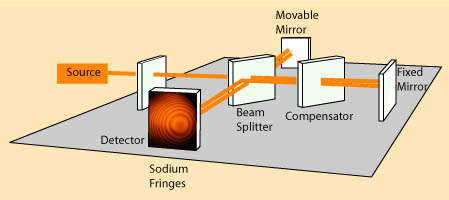
\includegraphics[width=.8\linewidth]{gfx/michel}
	\end{center}
\caption[Michelson Interferometer]{Michelson Interferometer \citep{michel:img}}\label{fig:michel}
\end{figure}
\par
Before complicating things, let us assume that the source of light is coherent and monochromatic. \marginpar{\Maggie Coherent means phase locked and Monochromatic means single frequency} Now in the \autoref{fig:michel}, we assume the source of light to be the light transmitted through the sample to be analysed. Say the interference at the detector is, at the given configuration, constructive. If we move the movable mirror by $\lambda / 4$, where $\lambda$ is the wavelength of the light, then the detector will receive a dark, destructive interference. If we plot the intensity at the detector as a function of displacement of the moveable mirror, we will, in this case, receive a sine wave.
\par
Now let us crank it up a notch. Let us consider the light to still be coherent, but not monochromatic. Let the source of light contain all the transmitted frequencies. \marginpar{\Lisa Note the fact that here, the measurement is simultaneous!} Now if the intensity is plotted against the displacement of the moveable mirror, we will get a superposition of sine waves, and we already know how to decompose them to find individual frequencies using \emph{Fourier Transformation}. This essentially gives us the spectrum, with wavenumber (dimensions of one over distance) on one axis, and intensity on the other.
\par
The source of infra-red light is a Silicon Carbide rod, that is heated to produce the desired radiations. \marginpar{\Bart How is SiC coherent?} The detector is capacitive, or so we were told. 
\subsection{Ultra Violet-Visible Spectroscopy}
